%%% Local Variables:
%%% mode: LaTeX
%%% TeX-master: "../../kr"
%%% End:


\subsection{Problems}


\subsubsection{Suppose Client A requests a web page from Server S through HTTP and its socket is associated with port 33000 (P1)}
It is assumed that ''its socket'' refers to S's socket for outgoing communication. \\
\\
\textbf{a. What are the source and destination ports for the segments sent from A to S?} \\
Since the segment is sent from A the source port must be whatever port the OS dynamically choses for sending HTTP. Since the segment is sent to S, then the destination port must be the port for S that handles HTTP, which is typically port 80. \\
\\
\textbf{b. What are the source and destination ports for the segments sent from S to A?} \\
Since the segment is sent from S the source port is S's port 330000. Since the segment is sent to A through HTTP, the destination port must be the port of A which handles HTTP, which is typically port 80. \\
\\ 
\textbf{c. Can Client A contact to Server S using UDP as the transport protocol?} \\
Usually HTTP is handled by TCP, but it can also be handled by UDP. This is for example the case in googles UDP based QUIC protocol. So yes, client A can contact server S using UDP.\\
\\
\textbf{d. Can Client A request multiple resources in a single TCP connection?} \\
Yes in a persistent connection it can. But not if it uses a non-persistent version of TCP, where each requested resource requires establishing a new TCP connection.


\subsubsection{Consider Figure 3.5. (P2)}

\textbf{a. Let us assume the following change: at B we want to access an FTP server from host A. What port number should be used to replace port 80?} \\
HTTP use port 80 while FTP use port 21, so the port number should be changed to 21. \\
\\
\textbf{b. Would there be an error if the right process of C used port number 8080?} \\
Port 8080 is commonly used as an alternative HTTP port for web servers and is mostly used for testing and development. Port 8080 is however in the unprivileged range and using it as a source port for an application will therefore not result in an error, so the answer is no. \\
\\
\textbf{c. What are the source and destination network and port values in the segments flowing from the server back to the clients' processes?} \\
\\
Segments flowing from the server back to client's is going to contain the source IP and port number of the server, which is not displayed on the figure.


\subsubsection{UDP and TCP use 1s complement for their checksums. Suppose you have the following three 16 bit words: 0101001101100110; 0111010010110100; \\ 0000110111000001. What is the 1s complement of the sum of these words? Show all work. Why is it that UDP offers a checksum? With the 1's complement scheme, how does the receiver detect errors? Describe how a single bit flip can be detected. (P3)}

Adding the first two words with wraparound overflow gives
\begin{equation*}
\begin{split}
    &0101 \, 0011 \, 0110 \, 0110 \\
    + &0111 \, 0100 \, 1011 \, 0100\\
    =  &1000 \, 1000 \, 0001 \, 1011
\end{split}
\end{equation*}
where overflow was wrapped around to the least significant digit. Adding the third word to the result gives
\begin{equation*}
\begin{split}
    &1000 \, 1000 \, 0001 \, 1011 \\
    + &0000 \, 1101 \, 1100 \, 0001 \\
    = & 1001 \, 0101 \, 1101 \, 1100
\end{split}
\end{equation*}
The 1s compliment of this number is $0110 \, 1010 \, 0010 \, 0011$, which is the checksum. \\
\\
UDP offers a checksum for error detection. With the 1s complement scheme the receiver can detect error by adding the 1-complimented checksum to the three bit words and if there is no errors the result should be all 1's by construction. But if a 0 is present in the result then it is clear that a bit-flip must have occurred during transfer. This scheme can however not detect all two-bit errors, since it might be possible that two bits were flipped in a way that the sum still contains only 1's.


\subsubsection{Assume that a host receives a UDP segment with 01011101 11110010 (we separated the values of each byte with a space for clarity) as the checksum. The host adds the 16-bit words over all necessary fields excluding the check-sum and obtains the value 00110010 00001101. Is the segment considered correctly received or not? What does the receiver do? (P4)}

No, it is not correctly received, because 0's present in the sum indicates bit-flip errors. Even though UDP provides this scheme for error detecting it does not provide ways to recover from these errors, so the receiver should not do anything.


\subsubsection{Suppose that the UDP receiver computes the Internet checksum for the received UDP segment and finds that it matches the value carried in the checksum field. Can the receiver be absolutely certain that no bit errors have occurred? Explain. (P5)}

No, one can not compare the computed checksum to the provided checksum and infer that no errors have occurred, because if two digits that should be added together in two words are 0 and 1 and these are both flipped then the checksum will remain the same. In that case there is clearly bit errors but none are detected. The receiver can only detect these if he adds the words and the checksum and check for the 1's.


\subsubsection{Consider our motivation for correcting protocol \texttt{rdt2.1.} Show that the receiver, shown in Figure 3.60, when operating with the sender shown in Figure 3.11, can lead the sender and receiver to enter into a deadlock state, where each is waiting for an event that will never occur. (P6)}
\label{sec:kr_3.9.6}

Say the sender in Figure 3.11 is in state ''wait for call 0 from above'' and receiver is in state ''Wait for 0 from below'' and the sender then sends the packet with sequence number 0. When the packet is received the receiver transitions to the state ''Wait for 1 from below'' and sends an ACK. Then if this ACK is corrupted then the sender will retransmit the packet with sequence number 0, but the sender is waiting for sequence number 1, so it will send a NAK. When the sender gets the NAK it will again resend the packet with sequence number 0, but again the receiver is waiting for sequence number 1 and will once again send a NAK. This is going to keep reoccurring; the receiver gets a packet with sequence number 0 and sends a NAK and this causes the sender to resend the packet with sequence number 0. Therefore the sender and receiver have entered a deadlock state.


\subsubsection{In protocol \texttt{rdt3.0}, the ACK packets flowing from the receiver to the sender do not have sequence numbers (although they do have an ACK field that contains the sequence number of the packet they are acknowledging). Why is it that our ACK packets do not require sequence numbers? (P7)}

\texttt{rdt3.0} does not need sequence numbers as it identifies the need to retransmit packets by having a countdown timer go down before receiving an ACK for the sent packet. It therefore only need to identify which ACks are for the recent packet and which are old duplicate ACKs and this is done by having alternating bits in the ACK field.


\subsubsection{Draw the FSM for the receiver side of protocol \texttt{rdt3.0}. (P8)}

From \texttt{rdt2.2} to \texttt{rdt3.0} there was only added the possibility of packet loss and the handling of such, but as this is solely handled by the sender via timeouts, the receiver is identical to the one in \texttt{rdt2.2}. Therefore we have that the receiver side of protocol \texttt{rdt3.0} can be drawn as the receiver of \texttt{rdt2.2} shown in Figure 3.13 of \cite{kr}.


\subsubsection{Give a trace of the operation of protocol \texttt{rdt3.0} when data packets and acknowledgment packets are garbled. Your trace should be similar to that used in Figure 3.16. (P9)}

''Garbled'' are interpreted as corrupted. Therefore the actions of sender and receiver in case of a garbled packet (acknowledgment) is identical to the actions in the case of a lost packet (acknowledgment) in Figure 3.16 except that the diagram should show the packet arriving but being corrupt. 


\subsubsection{Consider a channel that can lose packets but has a maximum delay that is known. Modify protocol \texttt{rdt2.1} to include sender timeout and retransmit. Informally argue why your protocol can communicate correctly over this channel. (P10)}

Add a timeout for the sender in \texttt{rdt2.1} that corresponds exactly to the time that the maximum delay is. If the there is a timeout before the sender has received an ACK or a NAK then it retransmits the last packet for which it has not received an ACK. This handles both the problem of the possible deadlock state shown in \ref{sec:kr_3.9.6} and also the problem with loss of ACKs.


\subsubsection{Consider the \texttt{rdt2.2} receiver in Figure 3.14, and the creation of a new packet in the self-transition (i.e., the transition from the state back to itself) in the Wait-for-0-from-below and the Wait-for-1-from-below states: \\ 
\texttt{sndpkt=make\_pkt(ACK,1,checksum)} and \texttt{sndpkt=make\_pkt(ACK,0,checksum)}. Would the protocol work correctly if this action were removed from the self-transition in the Wait-for-1-from-below state? Justify your answer. What if this event were removed from the self-transition in the Wait-for-0-from-below state? [Hint: In this latter case, consider what would happen if the first sender-to-receiver packet were corrupted.] (P11)}

No, the protocol would no longer work correctly, since the sender and receiver could then enter a deadlock state. This will happen if the sender sends a packet with seq 0 and enters ''wait for ACK 0'' and this packet gets lost while the receiver is in ''wait for 0 from below''. Since the receiver in this state no longer sends anything back to the sender, the sender will stay in its state and so will the receiver, thus arriving at at deadlock state.


\subsubsection{The sender side of \texttt{rdt3.0} simply ignores (that is, takes no action on)  all received packets that are either in error or have the wrong value in the acknum field of an acknowledgment packet. Suppose that in such circumstances, \texttt{rdt3.0} were simply to retransmit the current data packet. Would the protocol still work? (Hint: Consider what would happen if there were only bit errors; there are no packet losses but premature timeouts can occur. Consider how many times the nth packet is sent, in the limit as n approaches infinity.) (P12)}

Resending packets with errors immediately instead of waiting for a timeout would not change whether the protocol is working, since the same actions are taken, just prematurely. \\
\\
However if every packet with a wrong Acknum field is send prematurely we would have that every resend of such a packet would cause an Ack which would have the wrong value in the Acknum, which results in another resend and so on. This means that in a scenario where there are only bit errors but no packet loss (which could rid us of the extra ACKs), we would be sure that every bit error causes a resend that in turn causes an extra ACK and every such extra ACK causes another resend, meaning that the number of times packet $n$ is send will increase without bound as $n$ approaches infinity.


\subsubsection{Assume Host A is streaming a video from Server B using UDP. Also assume that the network suddenly becomes very congested while Host A is seeing the video. Is there any way to handle this situation with UDP? What about with TCP? Is there any other option? (P13)}

In a UDP streaming scenario, when the network becomes congested, there is no built-in mechanism to handle congestion control. UDP lacks flow control and error recovery mechanisms, so the quality of the video may degrade, and packets may be dropped. \\
\\
TCP, on the other hand, employs congestion control mechanisms. If the network becomes congested, TCP will adapt by reducing the transmission rate to alleviate the congestion. While this may cause buffering or delay in video playback, it helps avoid packet loss and ensures reliable delivery.


\subsubsection{Consider a stop-and-wait data-transfer protocol that provides error checking and retransmissions but uses only negative acknowledgments. Assume that negative acknowledgments are never corrupted. Would such a protocol work over a channel with bit errors? What about over a lossy channel with bit errors? (P14)}

Yes, if the acknowledgments are never corrupted and only the packets, then every corrupt packet will result in a negative ack, which is guaranteed to arrive at the sender and result in a retransmission. \\
\\
If the channel is also lossy, then the protocol no longer works as the negative acks can be lost and in such a case the sender will wait forever resulting in a deadlock state.


\subsubsection{Consider the cross-country example shown in Figure 3.17, with a 10 Gbps link. How big would the window size have to be for the channel utilization to be greater than 98 percent? Suppose that the size of a packet is 1,500 bytes, including header fields and data. (P15)}

The \textit{window size} is the number of packets that can be sent by the sender without receiving an acknowledgment. As in the example we have that the sender is transmitting for $\frac{L}{R} = \frac{1500 \cdot 8}{10^9} = 1.2 \cdot 10^{-5}$ seconds for each packet. Assuming negligible size of ACKs we have that the first ACK is received by the sender after RTT $+ 1.2 \cdot 10^{-5}$ seconds with $N$ being the window size (number of packets sent), at which time it can start sending packets again. We can therefore express the utilization as
\begin{equation*}
    U_{\text{sender}} = \frac{N \frac{L}{R}}{\text{RTT} + \frac{L}{R}}
\end{equation*} 
Isolating the window size $N$ gives
\begin{equation*}
\begin{split}
    U_{\text{sender}} &= \frac{N \frac{L}{R}}{\text{RTT} + \frac{L}{R}} \\
    U_{\text{sender}} \lr{\text{RTT} + \frac{L}{R}} &= N \frac{L}{R} \\
    N &= \frac{U_{\text{sender}} \lr{\text{RTT} + \frac{L}{R}}}{\frac{L}{R}}
\end{split}
\end{equation*}
Inserting the values (RTT is said to be 30 milliseconds in the example) we get
\begin{equation*}
    N = \frac{U_{\text{sender}} \lr{\text{RTT} + \frac{L}{R}}}{\frac{L}{R}} = \frac{ 0.98 \lr{30 \cdot 10^{-3} + 1.2 \cdot 10^{-5}}}{1.2 \cdot 10^{-5}} = 2450.98
\end{equation*}
So the channel utilization is greater than 0.98 for a window size of 2451.



\subsubsection{Suppose an application uses \texttt{rdt 3.0} as its transport layer protocol. As the stop-and-wait protocol has very low channel utilization (shown in the cross-country example), the designers of this application let the receiver keep sending back a number (more than two) of alternating ACK 0 and ACK 1 even if the corresponding data have not arrived at the receiver. Would this application design increase the channel utilization? Why? Are there any potential problems with this approach? Explain. (P16)}

Yes it would increase channel utilization as it pipelines packets. There is however one potential problem with the approach. If packets are lost then since the receiver sends alternating ACK 0 and ACK 1 even if data has not arrived, then the sender of \texttt{rdt 3.0} can not re-send the lost packets.


\subsubsection{Consider two network entities, A and B, which are connected by a perfect bi-directional channel (i.e., any message sent will be received correctly; the channel will not corrupt, lose, or re-order packets). A and B are to deliver data messages to each other in an alternating manner: First, A must deliver a message to B, then B must deliver a message to A, then A must deliver a message to B and so on. If an entity is in a state where it should not attempt to deliver a message to the other side, and there is an event like \texttt{rdt\_send(data)} call from above that attempts to pass data down for transmission to the other side, this call from above can simply be ignored with a call to \texttt{rdt\_unable\_to\_send(data)}, which informs the higher layer that it is currently not able to send data. [Note: This simplifying assumption is made so you don't have to worry about buffering data.] Draw a FSM specification for this protocol (one FSM for A, and one FSM for B!). Note that you do not have to worry about a reliability mechanism here; the main point of this question is to create a FSM specification that reflects the synchronized behavior of the two entities. You should use the following events and actions that have the same meaning as protocol \texttt{rdt1.0} in Figure 3.9: \texttt{rdt\_send(data)}, \texttt{packet = make\_pkt(data)}, \texttt{udt\_send(packet)}, \texttt{rdt\_rcv(packet)}, \texttt{extract (packet,data)}, \texttt{deliver\_data(data)}. Make sure your protocol reflects the strict alternation of sending between A and B. Also, make sure to indicate the initial states for A and B in your FSM descriptions. (P17)}

FSM for A:
\begin{center}
\begin{tikzpicture}[node distance=7cm]
    \node[state, initial, text width=2cm] (snd) {Wait to send packet to B};
    \node[state, right of=snd, text width=2cm] (rcv) {Wait to receive packet from B};

    \draw (snd) edge[loop above] node {$\frac{\texttt{rdt\_send(data)}}{\texttt{rdt\_unable\_to\_send(data)}}$} (snd);
    \draw (rcv) edge[loop below] node {$\frac{\texttt{rdt\_send(data)}}{\texttt{rdt\_unable\_to\_send(data)}}$} (rcv);
    \draw (snd) edge[bend left, above] node {$\frac{\texttt{rdt\_send(data)}}{\texttt{packet=make\_pkt(data), udt\_send(packet)}}$} (rcv);
    \draw (rcv) edge[bend left, below] node {$\frac{\texttt{rdt\_receive(data)}}{\texttt{extract(packet, data), deliver\_data(data)}}$} (snd);
\end{tikzpicture}    
\end{center}
FSM for B:
\begin{center}
\begin{tikzpicture}[node distance=1cm]
    \node[state, right of=rcv, text width=2cm] (snd) {Wait to send packet to B};
    \node[state, initial, text width=2cm] (rcv) {Wait to receive packet from B};

    \draw (snd) edge[loop above] node {$\frac{\texttt{rdt\_send(data)}}{\texttt{rdt\_unable\_to\_send(data)}}$} (snd);
    \draw (rcv) edge[loop below] node {$\frac{\texttt{rdt\_send(data)}}{\texttt{rdt\_unable\_to\_send(data)}}$} (rcv);
    \draw (snd) edge[bend left, above] node {$\frac{\texttt{rdt\_send(data)}}{\texttt{packet=make\_pkt(data), udt\_send(packet)}}$} (rcv);
    \draw (rcv) edge[bend left, below] node {$\frac{\texttt{rdt\_receive(data)}}{\texttt{extract(packet, data), deliver\_data(data)}}$} (snd);
\end{tikzpicture}    
\end{center}


\subsubsection{In the generic SR protocol that we studied in Section 3.4.4, the sender transmits a message as soon as it is available (if it is in the window) without waiting for an acknowledgment. Suppose now that we want an SR protocol that sends messages two at a time. That is, the sender will send a pair of messages and will send the next pair of messages only when it knows that both messages in the first pair have been received correctly. Suppose that the channel may lose messages but will not corrupt or reorder messages. Design an error-control protocol for the unidirectional reliable transfer of messages. Give an FSM description of the sender and receiver. Describe the format of the packets sent between sender and receiver, and vice versa. If you use any procedure calls other than those in Section 3.4  (for example, \texttt{udt\_send()}, \texttt{start\_timer()}, \texttt{rdt\_rcv()}, and so on), clearly state their actions. Give an example (a timeline trace of sender and receiver) showing how your protocol recovers from a lost packet. (P18)}

The sender waits until it receives an ACK for a pair of messages (seqnum and seqnum + 1) before moving on to the next pair. Data packets have a data field with a two-bit sequence number, so that we can express the sequence numbers 0, 1, 2 and 3. Four distinct sequence numbers are necessary to distinguish in which pair of messages that might have been lost. \\
\\
The sender state records whether:
\begin{itemize}
    \item No ACKs have been received for the current pair
    \item Only an ACK for seqnum and not seqnum + 1 has been received.
    \item Only an ACK for seqnum + 1 and not seqnum has been received.
\end{itemize}
It is assumed that seqnum is initially 0 and that the sender has sent the first two data messages. \\
\\
FSM for the sender: \\
\begin{center}
\begin{tikzpicture}[node distance=7cm]
    \node[state, text width=2cm] (pair) {Wait for pair of ACKs};
    \node[state, above right of=pair, text width=2cm] (odd) {Wait for odd ACK};
    \node[state, below right of=pair, text width=2cm] (even) {Wait for even ACKs};

    \draw (pair) edge[out=110, in=520, looseness=3] node[above] {$
        \frac{
            \parbox{2.5in \scriptsize}{($\texttt{rdt\_rcv(rcvpkt)} \&\& \texttt{corrupt(rcvpkt)})$ \\
            $||$ \\
            $\lr{ \texttt{rdt\_rcv(rcvpkt)} \&\& \texttt{notcorrupt(rcvpkt)}}$ \\
            $ \& \& \texttt{has\_not\_ACK(seqnum)} \& \& \texttt{has\_not\_ACK(seqnum + 1)}$
            }}{
        }
    $} (pair);
    \draw (pair) edge[out=550, in=600, looseness=3] node[below] {$
        \frac{
            \texttt{timeout}
            }{
                \parbox{1.5in \scriptsize}{$\texttt{udt\_send(sndpkt, seqnum)}$ \\
                $\texttt{udt\_send(sndpkt, seqnum + 1)}$ \\
                $\texttt{start\_timer}$
            }}$
    } (pair);

    \draw (odd) edge[out=50, in=0, looseness=3] node[right] {$
        \frac{
            \texttt{timeout}
        }{\parbox{1.5in \scriptsize}{
            $\texttt{udt\_send(sndpkt, seqnum + 1)}$ \\
            $\texttt{start\_timer}$
        }}$} (odd);
    \draw (odd) edge[out=-60, in=-10, looseness=3] node[right] {$
        \frac{\parbox{2in \scriptsize}{
            $\texttt{\texttt{rdt\_rcv(rcvpkt)}} \& \& \texttt{notcorrupt(rcvpkt)}$ \\
            $ \& \& \texttt{has\_ack(seqnum)}$ \\
            $|| (\texttt{rdt\_rcv(rcvpkt)} \& \& \texttt{corrupt(rcvpkt)})$
            }}{
            }$} (odd);

    \draw (even) edge[out=50, in=0, looseness=3] node[right] {$
        \frac{\parbox{2in \scriptsize}{
            $\texttt{(\texttt{rdt\_rcv(rcvpkt)} \& \& notcorrupt(rcvpkt)}$ \\
            $\& \& \texttt{has\_ack(seqnum + 1))}$ \\
            $|| (\texttt{rdt\_rcv(rcvpkt)} \& \& \texttt{corrupt(rcvpkt)})$
            }}{
        }$} (even);
    \draw (even) edge[out=-60, in=-10, looseness=3] node[right] {$
    \frac{
        \texttt{timeout}
    }{\parbox{1.3in \scriptsize}{
        $\texttt{udt\_send(sndpkt, seqnum)}$ \\
        $\texttt{start\_timer}$   
    }}$} (even);

    \draw (pair) edge[bend left, above] node[above] {$
    \frac{\parbox{1.2in \scriptsize}{
        $\texttt{rdt\_rcv(rcvpkt)}$ \\
        $\& \& \texttt{notcorrupt(rcvpkt)}$ \\
        $\& \& \texttt{has\_ack(seqnum)}$
    }}{
    }$} (odd);
    \draw (odd) edge[bend left, below] node[below] {$
    \frac{\parbox{2in \scriptsize}{
        $\texttt{rdt\_rcv(rcvpkt)$ \\ 
        $\& \& notcorrupt(rcvpkt)}$ \\
        $\& \& \texttt{has\_ack(seqnum + 1)}$
    }}{\parbox{2in \scriptsize}{
        $\texttt{seqnum = seqnum + 2}$ \\
        $\texttt{udt\_send(sndpkt, seqnum)}$ \\
        $\texttt{udt\_send(sndpkt, seqnum + 1)}$ \\
        $\texttt{start\_timer}$
    }}$} (pair);

    \draw (pair) edge[bend left, above] node[above] {$
    \frac{\parbox{1.2in \scriptsize}{
        $\texttt{rdt\_rcv(rcvpkt)}$ \\
        $\& \& \texttt{notcorrupt(rcvpkt)}$ \\
        $\& \& \texttt{has\_ack(seqnum+1)}$
    }}{
    }$} (even);
    \draw (even) edge[bend left, below] node[below] {$
    \frac{\parbox{1.8in \scriptsize}{
        $\texttt{rdt\_rcv(rcvpkt)$ \\
        $\& \& \texttt{notcorrupt(rcvpkt)}}$ \\
        $\& \& \texttt{has\_ack(seqnum)}$
    }}{\parbox{2in \scriptsize}{
        $\texttt{seqnum = seqnum + 2}$ \\
        $\texttt{udt\_send(sndpkt, seqnum)}$ \\   
        $\texttt{udt\_send(sndpkt, seqnum + 1)}$ \\
        $\texttt{start\_timer}$  
    }}$} (pair);
\end{tikzpicture}    
\end{center}
FSM for the receiver:
\begin{center}
    \begin{tikzpicture}[node distance=7cm]
        \node[state, text width=2cm] (pair) {Wait for pair of data};
        \node[state, above right of=pair, text width=2cm] (odd) {Wait for odd data};
        \node[state, below right of=pair, text width=2cm] (even) {Wait for even data};
    
        \draw (pair) edge[out=110, in=520, looseness=3] node[above] {$
            \frac{\parbox{1.8in \scriptsize}{
                ($\texttt{rdt\_rcv(rcvpkt)} \&\& \texttt{corrupt(rcvpkt)})$ 
                }}{
            }
        $} (pair);
        \draw (pair) edge[out=550, in=600, looseness=3] node[below] {$
            \frac{\parbox{1.5in \scriptsize}{
                $\texttt{rdt\_rcv(rcvpkt)} \& \& \texttt{notcorrupt(rcvpkt)}$ \\
                $\& \& \texttt{has\_seq(x)}$ \\
                $\& \& \texttt{x != seqnum}$ \\
                $\& \& \texttt{x != seqnum + 1}$
                }}{\parbox{1.5in \scriptsize}{
                    $\texttt{udt\_send(ACK, x)}$ \\
                }}$
        } (pair);
    
        \draw (odd) edge[out=50, in=0, looseness=3] node[right] {$
            \frac{
                \texttt{rdt\_rcv(rcvpkt)} \& \& \texttt{corrupt(rcvpkt)}
            }{\parbox{1.5in \scriptsize}{
            }}$} (odd);
        \draw (odd) edge[out=-60, in=-10, looseness=3] node[right] {$
            \frac{\parbox{1.9in \scriptsize}{
                $\texttt{\texttt{rdt\_rcv(rcvpkt)}} \& \& \texttt{notcorrupt(rcvpkt)}$ \\
                $ \& \& \texttt{has\_seq(seqnum + 1)}$ 
                }}{
                    \texttt{udt\_send(ACK, seqnum)}
                }$} (odd);
    
        \draw (even) edge[out=50, in=0, looseness=3] node[right] {$
            \frac{\parbox{2in \scriptsize}{
                $\texttt{\texttt{rdt\_rcv(rcvpkt)} \& \& notcorrupt(rcvpkt)}$ \\
                $\& \& \texttt{has\_seq(seqnum + 1)}$
                }}{
                    \texttt{udt\_send(ACK, seqnum + 1)}
            }$} (even);
        \draw (even) edge[out=-60, in=-10, looseness=3] node[right] {$
        \frac{
            \texttt{rdt\_rcv(rcvpkt)} \& \& \texttt{corrupt(rcvpkt)}
        }{
        }$} (even);
    
        \draw (pair) edge[bend left, above] node[above] {$
        \frac{\parbox{2in \scriptsize}{
            $\texttt{rdt\_rcv(rcvpkt)$ \\ 
            $\& \& notcorrupt(rcvpkt)}$ \\
            $\& \& \texttt{has\_seq(seqnum)}$
        }}{\parbox{2in \scriptsize}{
            $\texttt{udt\_send(ACK, seqnum)}$ 
        }}$} (odd);
        \draw (odd) edge[bend left, below] node[below] {$
        \frac{\parbox{1.2in \scriptsize}{
            $\texttt{rdt\_rcv(rcvpkt)}$ \\
            $\& \& \texttt{notcorrupt(rcvpkt)}$ \\
            $\& \& \texttt{has\_seq(seqnum + 1)}$
        }}{\parbox{1.2in \scriptsize}{
            $\texttt{udt\_send(ACK, seqnum + 1)}$ \\
            $\texttt{seqnum = seqnum + 2}$
        }}$} (pair);
    
        \draw (pair) edge[bend left, above] node[above] {$
        \frac{\parbox{1.2in \scriptsize}{
            $\texttt{rdt\_rcv(rcvpkt)}$ \\
            $\& \& \texttt{notcorrupt(rcvpkt)}$ \\
            $\& \& \texttt{has\_seq(seqnum+1)}$
        }}{
            \texttt{udt\_send(ACK, seqnum + 1)}
        }$} (even);
        \draw (even) edge[bend left, below] node[below] {$
        \frac{\parbox{1.8in \scriptsize}{
            $\texttt{rdt\_rcv(rcvpkt)$ \\
            $\& \& \texttt{notcorrupt(rcvpkt)}}$ \\
            $\& \& \texttt{has\_seq(seqnum)}$
        }}{\parbox{2in \scriptsize}{
            $\texttt{udt\_send(ACK, seqnum)}$ \\  
            $\texttt{seqnum = seqnum + 2}$ \\  
        }}$} (pair);
\end{tikzpicture}    
\end{center}
Timing diagram:

\begin{tikzpicture}[node distance=4cm,auto,>=stealth']
    \node[] (receiver) {receiver};
    \node[left = of receiver] (sender) {sender};
    \node[below of=receiver, node distance=5cm] (receiver_ground) {};
    \node[below of=sender, node distance=5cm] (sender_ground) {};
    %
    \draw (sender) -- (sender_ground);
    \draw (receiver) -- (receiver_ground);
    \draw[->, red] ($(sender)!0.1!(sender_ground)$) -- node[above,scale=0.7, midway]{make pair (0,1), send packet 0, loss} (-0.6, -0.9);
    \draw[->] ($(sender)!0.25!(sender_ground)$) -- node[above,scale=0.7, midway]{send pkt1} ($(receiver)!0.4!(receiver_ground)$);
    \draw[<-] (-0.9, -2.8) -- node[above,scale=0.7,midway]{send ACK1} ($(receiver)!0.4!(receiver_ground)$);
    \draw[->] ($(sender)!0.6!(sender_ground)$) -- node[above,scale=0.7, midway]{timeout, resend packet 0} ($(receiver)!0.8!(receiver_ground)$);
    \draw[<-] (-0.9, -4.8) -- node[above,scale=0.7,midway]{send ACK0, deliver pair (0, 1)} ($(receiver)!0.8!(receiver_ground)$);
\end{tikzpicture}



\subsubsection{Suppose Host A and Host B use a GBN protocol with window size $N = 3$ and a long-enough range of sequence numbers. Assume Host A sends six application messages to Host B and that all messages are correctly received, except for the first acknowledgment and the fifth data segment. Draw a timing diagram (similar to Figure 3.22), showing the data segments and the acknowledgments sent along with the corresponding sequence and acknowledge numbers, respectively. (P19)}

\begin{tikzpicture}[node distance=4cm,auto,>=stealth']
    \node[] (receiver) {receiver};
    \node[left = of receiver] (sender) {sender};
    \node[below of=receiver, node distance=15cm] (receiver_ground) {};
    \node[below of=sender, node distance=15cm] (sender_ground) {};
    %
    \draw (sender) -- (sender_ground);
    \draw (receiver) -- (receiver_ground);
    \draw[->] ($(sender)!0.02!(sender_ground)$) -- node[above,scale=0.7, midway]{send pkt0} ($(receiver)!0.05!(receiver_ground)$);
    \draw[<-, red] (-0.5, -0.9) -- node[above,scale=0.7,midway]{send ACK0, loss} ($(receiver)!0.05!(receiver_ground)$);
    \draw[->] ($(sender)!0.05!(sender_ground)$) -- node[above,scale=0.7, midway]{send pkt1} ($(receiver)!0.1!(receiver_ground)$);
    \draw[<-] (-0.9, -1.8) -- node[above,scale=0.7,midway]{send ACK1} ($(receiver)!0.1!(receiver_ground)$);
    \draw[->] ($(sender)!0.1!(sender_ground)$) -- node[above,scale=0.7, midway]{send pkt2, wait} ($(receiver)!0.15!(receiver_ground)$);
    \draw[<-] (-0.9, -2.8) -- node[above,scale=0.7,midway]{send ACK2} ($(receiver)!0.15!(receiver_ground)$);
    \draw[->] ($(sender)!0.15!(sender_ground)$) -- node[above,scale=0.7, midway]{pkt0 timeout, send pkt 0} ($(receiver)!0.2!(receiver_ground)$);
    \draw[<-] ($(sender)!0.3!(sender_ground)$) -- node[above,scale=0.7,midway]{discard, send ACK0} ($(receiver)!0.2!(receiver_ground)$);
    \draw[->, red] ($(sender)!0.2!(sender_ground)$) -- node[above,scale=0.7, midway]{send pkt 1, loss} (-3, -3.3);
    \draw[->] ($(sender)!0.25!(sender_ground)$) -- node[above,scale=0.7, midway]{send pkt2, wait} ($(receiver)!0.3!(receiver_ground)$);
    \draw[<-] (-0.9, -5.0) -- node[above,scale=0.7,midway]{discard, send ACK2} ($(receiver)!0.3!(receiver_ground)$);
    \draw[->] ($(sender)!0.3!(sender_ground)$) -- node[above,scale=0.7, midway]{send pkt3, wait} ($(receiver)!0.35!(receiver_ground)$);
    \draw[<-] (-0.9, -5.8) -- node[above,scale=0.7,midway]{send ACK3} ($(receiver)!0.35!(receiver_ground)$);
    \draw[->] ($(sender)!0.4!(sender_ground)$) -- node[above,scale=0.7, midway]{pkt1 timeout send pkt1} ($(receiver)!0.45!(receiver_ground)$);
    \draw[<-] ($(sender)!0.65!(sender_ground)$) -- node[above,scale=0.7,midway]{discard, send ACK1} ($(receiver)!0.45!(receiver_ground)$);
    \draw[->] ($(sender)!0.45!(sender_ground)$) -- node[above,scale=0.7, midway]{send pkt2} ($(receiver)!0.50!(receiver_ground)$);
    \draw[<-] ($(sender)!0.70!(sender_ground)$) -- node[above,scale=0.7,midway]{discard, send ACK2} ($(receiver)!0.50!(receiver_ground)$);
    \draw[->] ($(sender)!0.50!(sender_ground)$) -- node[above,scale=0.7, midway]{send pkt3, wait} ($(receiver)!0.55!(receiver_ground)$);
    \draw[<-] ($(sender)!0.75!(sender_ground)$) -- node[above,scale=0.7,midway]{discard, send ACK3} ($(receiver)!0.55!(receiver_ground)$);
    \draw[->] ($(sender)!0.65!(sender_ground)$) -- node[above,scale=0.7, midway]{send pkt4, wait} ($(receiver)!0.70!(receiver_ground)$);
    \draw[<-] ($(sender)!0.85!(sender_ground)$) -- node[above,scale=0.7,midway]{send ACK4} ($(receiver)!0.70!(receiver_ground)$);
    \draw[->] ($(sender)!0.70!(sender_ground)$) -- node[above,scale=0.7, midway]{send pkt5} ($(receiver)!0.75!(receiver_ground)$);
    \draw[<-] ($(sender)!0.90!(sender_ground)$) -- node[above,scale=0.7,midway]{send ACK5} ($(receiver)!0.75!(receiver_ground)$);
\end{tikzpicture}



\subsubsection{Consider a scenario in which Host A and Host B want to send messages to Host C. Hosts A and C are connected by a channel that can lose and corrupt (but not reorder) messages. Hosts B and C are connected by another channel (independent of the channel connecting A and C) with the same properties. The transport layer at Host C should alternate in delivering messages from  A and B to the layer above (that is, it should first deliver the data from a packet from A, then the data from a packet from B, and so on). Design a stop-and-wait-like error-control protocol for reliably transferring packets from A and B to C, with alternating delivery at C as described above. Give FSM descriptions of A and C. (Hint: The FSM for B should be essentially the same as  for A.) Also, give a description of the packet format(s) used. (P20)}

\begin{center}
    \begin{tikzpicture}[node distance=6cm]
        \node[state, text width=1.4cm] (0A) {Wait for 0 from A};
        \node[state, right of=0A, text width=1.4cm] (0B) {Wait for 0 from B};
        \node[state, below of=0A, text width=1.4cm] (1B) {Wait for 1 from B};
        \node[state, right of=1B, text width=1.4cm] (1A) {Wait for 1 from A};
    
        \draw (0A) edge[out=110, in=520, looseness=3] node[left] {$
            \frac{\parbox{1.8in \scriptsize}{
                $\texttt{rdt\_rcv(rcvpkt)} \&\& \texttt{from\_B(rcvpkt)}$ 
                }}{
                    \Lambda
            }
        $} (0A);
        \draw (0A) edge[out=590, in=540, looseness=3] node[left] {$
            \frac{\parbox{1.8in \scriptsize}{
                $\texttt{rdt\_rcv(rcvpkt)} \& \& \texttt{corrupt(rcvpkt)}$ \\
                $|| \texttt{has\_seq1(rcvpkt)} \& \& \texttt{from\_A(rcvpkt)}$
                }}{\parbox{1.8in \scriptsize}{
                    $\texttt{sndpkt=make\_pkt(ACK, 1, checksum)}$ \\
                    $\texttt{udt\_send(A, sndpkt)}$
                }}$
        } (0A);
    
        \draw (0B) edge[out=110, in=60, looseness=3] node[right] {$
            \frac{
                \texttt{rdt\_rcv(rcvpkt)} \& \& \texttt{from\_A(rcvpkt)}
            }{
                \Lambda
            }$} (0B);
        \draw (0B) edge[out=0, in=50, looseness=3] node[right] {$
            \frac{\parbox{1.3in \tiny}{
                $\texttt{\texttt{rdt\_rcv(rcvpkt)}} \& \& \texttt{corrupt(rcvpkt)}$ \\
                $ || \texttt{has\_seq1(rcvpkt)} \& \& \texttt{from\_B(rcvpkt)}$ 
                }}{\parbox{1.3in \tiny}{
                    $\texttt{sndpkt=make\_pkt(ACK, 1, checksum)}$ \\
                    $\texttt{udt\_send(B, sndpkt)}$
                }}$} (0B);
    
        \draw (1A) edge[out=50, in=0, looseness=3] node[right] {$
            \frac{\parbox{1.3in \tiny}{
                $\texttt{\texttt{rdt\_rcv(rcvpkt)} \& \& corrupt(rcvpkt)}$ \\
                $|| \texttt{has\_seq0(rcvpkt)} \& \& \texttt{from\_A(rcvpkt)}$
                }}{\parbox{1.3in \tiny}{
                    $\texttt{sndpkt = make\_pkt(ACK, 0, checksum)}$ \\
                    $\texttt{udt\_send(A, sndpkt)}$
                }}$} (1A);
        \draw (1A) edge[out=-60, in=-10, looseness=3] node[below] {$
        \frac{
            \texttt{rdt\_rcv(rcvpkt)} \& \& \texttt{from\_A(rcvpkt)}
        }{
            \Lambda
        }$} (1A);

        \draw (1B) edge[out=-80, in=-130, looseness=3] node[left] {$
            \frac{\parbox{1.9in \scriptsize}{
                $\texttt{\texttt{rdt\_rcv(rcvpkt)} \& \& corrupt(rcvpkt)}$ \\
                $|| \texttt{has\_seq0(rcvpkt)} \& \& \texttt{from\_B(rcvpkt)}$
                }}{\parbox{1.9in \scriptsize}{
                    $\texttt{sndpkt = make\_pkt(ACK, 0, checksum)}$ \\
                    $\texttt{udt\_send(B, sndpkt)}$
                }}$} (1B);
        \draw (1B) edge[out=-140, in=-190, looseness=3] node[left] {$
        \frac{
            \texttt{rdt\_rcv(rcvpkt)} \& \& \texttt{from\_A(rcvpkt)}
        }{
            \Lambda
        }$} (1B);
    
        \draw (0A) edge[bend left, above] node[above] {$
        \frac{\parbox{2in \scriptsize}{
            $\texttt{rdt\_rcv(rcvpkt) \& \& notcorrupt(rcvpkt)}$ \\
            $\& \& \texttt{has\_seq0(rcvpkt)} \& \& \texttt{from\_A(rcvpkt)}$
        }}{\parbox{2in \scriptsize}{
            $\texttt{extract(rcvpkt, data)}$ \\
            $\texttt{deliver\_data(data)}$ \\
            $\texttt{sndpkt = make\_pkt(ACK, 0, checksum)}$ \\
            $\texttt{udt\_send(A, sndpkt)}$
        }}$} (0B);
        
        \draw (0B) edge[bend left, above] node[left] {$
        \frac{\parbox{2in \scriptsize}{
            $\texttt{rdt\_rcv(rcvpkt) \& \& notcorrupt(rcvpkt)}$ \\
            $\& \& \texttt{has\_seq0(rcvpkt)} \& \& \texttt{from\_B(rcvpkt)}$
        }}{\parbox{2in \scriptsize}{
            $\texttt{extract(rcvpkt, data)}$ \\
            $\texttt{deliver\_data(data)}$ \\
            $\texttt{sndpkt = make\_pkt(ACK, 0, checksum)}$ \\
            $\texttt{udt\_send(B, sndpkt)}$
        }}$} (1A);

        \draw (1A) edge[bend left, above] node[below] {$
        \frac{\parbox{2in \scriptsize}{
            $\texttt{rdt\_rcv(rcvpkt) \& \& notcorrupt(rcvpkt)}$ \\
            $\& \& \texttt{has\_seq1(rcvpkt)} \& \& \texttt{from\_A(rcvpkt)}$
        }}{\parbox{2in \scriptsize}{
            $\texttt{extract(rcvpkt, data)}$ \\
            $\texttt{deliver\_data(data)}$ \\
            $\texttt{sndpkt = make\_pkt(ACK, 1, checksum)}$ \\
            $\texttt{udt\_send(A, sndpkt)}$
        }}$} (1B);

        \draw (1B) edge[bend left, above] node[left] {$
        \frac{\parbox{2in \scriptsize}{
            $\texttt{rdt\_rcv(rcvpkt) \& \& notcorrupt(rcvpkt)}$ \\
            $\& \& \texttt{has\_seq1(rcvpkt)} \& \& \texttt{from\_B(rcvpkt)}$
        }}{\parbox{2in \scriptsize}{
            $\texttt{extract(rcvpkt, data)}$ \\
            $\texttt{deliver\_data(data)}$ \\
            $\texttt{sndpkt = make\_pkt(ACK, 1, checksum)}$ \\
            $\texttt{udt\_send(B, sndpkt)}$
        }}$} (0A);
\end{tikzpicture}    
\end{center}




\subsubsection{Suppose we have two network entities, A and B. B has a supply of data messages that will be sent to A according to the following conventions. When A gets a request from the layer above to get the next data (D) message from B, A must send a request (R) message to B on the A-to-B channel. Only when B receives an R message can it send a data (D) message back to A on the B-to-A channel. A should deliver exactly one copy of each D message to the layer above. R messages can be lost (but not corrupted) in the A-to-B channel; D messages, once sent, are always delivered correctly. The delay along both channels is unknown and variable. Design (give an FSM description of) a protocol that incorporates the appropriate mechanisms to compensate for the loss-prone A-to-B channel and implements message passing to the layer above at entity A, as discussed above. Use only those mechanisms that are absolutely necessary. (21)}

Due to potential message loss in the A-to-B channel, A may need to retransmit its requests and could inadvertently send duplicate requests due to variable and unknown channel delays. To detect duplicates, the protocol employs sequence numbers, where a 1-bit sequence number suffices for a stop-and-wait type of protocol. \\
\\
A (the requestor) operates in four states:
\begin{enumerate}
    \item \textbf{"Wait for Request 0 from above"}: A waits for a request from above to send a data unit. Upon receiving the request, it sends a request message (R0) to B, starts a timer, and transitions to the "Wait for D0" state. It disregards anything received from B in this state.
    \item \textbf{"Wait for D0"}: A waits for a D0 data message from B, with a running timer. If the timer expires, A resends an R0 message, restarts the timer, and stays in this state. Upon receiving a D0 message, A stops the timer and transitions to "Wait for Request 1 from above". D1 messages received in this state are ignored.
    \item \textbf{"Wait for Request 1 from above"}: A waits for another request from above. Upon receiving it, it sends a request message (R1) to B, starts a timer, and transitions to "Wait for D1". It ignores messages from B in this state.
    \item \textbf{"Wait for D1"}: A waits for a D1 data message from B, with a running timer. If the timer expires, A resends an R1 message, restarts the timer, and stays in this state. Upon receiving a D1 message, A stops the timer and transitions to "Wait for Request 0 from above". D0 messages received in this state are ignored.
\end{enumerate}

The data supplier (B) operates in two states:
\begin{enumerate}
    \item \textbf{"Send D0"}: B responds to R0 messages by sending D0 and remains in this state. Upon receiving an R1 message, it discards the D0 data (since it's already been received) and transitions to "Send D1" to send the next requested data piece.
    \item \textbf{"Send D1"}: B responds to R1 messages by sending D1 and remains in this state. Upon receiving another R1 message, it transitions back to "Send D1".
\end{enumerate}



\subsubsection{Consider the GBN protocol with a sender window size of 4 and a sequence number range of 1,024. Suppose that at time $t$, the next in-order packet that the receiver is expecting has a sequence number of $k$. Assume that the medium does not reorder messages. Answer the following questions: (P22)}

\textbf{a. What are the possible sets of sequence numbers inside the sender's window at time $t$? Justify your answer.} \\
If the receiver have received and ACKed the preceding $k-1$ packets and these ACKs have been received by the sender, then the sender's window is $[k, k - 1 + N]$, where $N$ is the window size. Since $N = 4$ we have $[k, k + 3]$. \\
\\
If no ACKs from preceding $k - 1$ packets have been received by the sender, then the sender's window is $[k - N, k - 1]$ in the general case and in our case $[k - 4, k - 1]$.
\\
Since these are the two extremes of the sets of sequence numbers we can combine the end points for these intervals and the possible sets of sequence numbers in the sender's window will be $[k - N, k - 1 + N]$. \\
\\
\textbf{b. What are all possible values of the ACK field in all possible messages currently propagating back to the sender at time $t$? Justify your answer.} \\
If the receiver have received and ACKed the preceding $k - 1$ packets then the earliest ACK will be $k - 1 - N$, since this is what is limited by a window size of $N$, and the latest ACK will be $k - 1$. So the propagating ACKs will have values in the range $[k - 1 - N, k - 1]$ which in our case with $N = 4$ is $[k - 5, k - 1]$.



\subsubsection{Give one example where buffering out-of-order segments would significantly improve the throughput of a GBN protocol. (P23)}

If a segment is delivered to the receiver but the corresponding ACK is lost. Then the proceeding segments that are send and ACKed are not buffered at thus decreases throughput significantly especially if the timeout is long and the window large.



\subsubsection{Consider a scenario where the three hosts A, B, and C are connected as a ring: A to B, B to C, and C to A. Assume that A and C run protocol \texttt{rdt3.0}, whereas B simply relays all messages received from A to C. (P24)}

\textbf{a. Does this arrangement enable reliable delivery of messages from A to C?} \\
When A transmits through B to C every mechanism (timeout and ACKs) that enable reliable data delivery are retransmitted by B, as they would be any node in the network, and therefore still works as intended, however timeout must account for the extra RTT that B introduces. \\
\\
Since C sends directly to A we have the case of 2 hosts that sends using \texttt{rdt3.0} which has reliable data transfer. Since B does not transmit data but simply relays it, we have no other cases to consider. Therefore we have that this arrangement enables reliable data transfer. \\
\\
\textbf{b. Can B tell if a certain message has been correctly received by A?} \\
\\
If A has received a message from C then it has been sent directly whereafter the ACK will be sent through B to C. Therefor B will know by receiving the ACK whether A has correctly received a message.



\subsubsection{We have said that an application may choose UDP for a transport protocol because UDP offers finer application control (than TCP) of what data is sent in a segment and when. (P25)}

\textbf{Why does an application have more control of what data is sent in a segment?} \\
In UDP the application have more control of the data sent in the segment, since a segment in UDP mostly contains the application data and not all the extra data that TCP adds for reliable data transfer and congestion control.\\
\\
\textbf{Why does an application have more control on when the segment is sent?} \\
Because UDP sends segments as soon as the application layer has handed its package to UDP. TCP on the other hand needs handshaking before sending and holds segments in a buffer before sending to implement reliable data transfer and congestion control.\\


\subsubsection{Consider transferring an enormous file of $L$ bytes from Host A to Host B. Assume an MSS of 536 bytes. (P26)}

\textbf{a. What is the maximum value of $L$ such that TCP sequence numbers are not exhausted? Recall that the TCP sequence number field has 4 bytes.} \\
Since TCP sequence number field has 4 bytes it can express $2^{4 \cdot 8} = 2^{32} = 4 \, 294 \, 967 \, 296$ numbers. Since the sequence numbers are incremented by the bytes of data sent the MSS is irrelevant, and $L$ is only limited by having fewer than $2^{32}$ bytes. \\
\\
\textbf{b. For the $L$ you obtain in (a), find how long it takes to transmit the file. Assume that a total of 66 bytes of transport, network, and data-link header are added to each segment before the resulting packet is sent out over a 155 Mbps link. Ignore flow control and congestion control so A can pump out the segments back to back and continuously.} 
\\
Since MSS is strictly the payload, we have that each segment is $536 + 66 = 602$ bytes. Since $L$ can max be $2^{32}$ we have that we must send $\ceil{\frac{2^{32}}{536}} = 8 \, 012 \,999$ segments for the total file to be transferred. Each of these segments are transferred over the 155 Mbps link in $\frac{602 \cdot 8 \, \text{bits}}{155 \cdot 10^6 \, \text{bits/s}} = 3.1 \cdot 10^{-5}$ seconds. This means that the whole file will be transferred in $8 \, 012 \, 999 \cdot 3.1 \cdot 10^{-5} = 248$ seconds.


\subsubsection{Host A and B are communicating over a TCP connection following RFC 5681. Host B has already received from A all bytes up through byte 96. Suppose Host A then sends two segments to Host B back-to-back. The first and the second segments contain 40 and 80 bytes of data, respectively. In the first segment, the sequence number is 97, the source port number is 302, and the destination port number is 80. Host B sends an acknowledgment whenever it receives a segment from Host A. (P27)}

\textbf{a. In the second segment sent from Host A to B, what are the sequence number, source port number, and destination port number?} \\
Since the first segment has sequence number 97 and contains 40 bytes of data then the receiver must afterwards have received bytes up through byte $96 + 40 = 136$. Therefore the first byte in the second segment will be byte 137 of the byte stream and therefore the sequence number for the second segment must be 137. \\
\\
The port numbers are identical to the ones for the first segment so the source port number is 302 and the destination port number is 80.
\\
\textbf{b. If the first segment arrives before the second segment, in the acknowledgment of the first arriving segment, what is the acknowledgment number, the source port number, and the destination port number?} \\
Acknowledgment numbers indicate the expected sequence number of the next package. Therefore the acknowledgment number for the first segment will be the sequence number for the second package which is 137.\\
\\
Since acknowledgments come from the receiver the port numbers have changed roles and therefore the source port number is 80 and the destination port number is 302. \\
\\
\textbf{c. If the second segment arrives before the first segment, in the acknowledgment of the first arriving segment, what is the acknowledgment number?} \\
If the second segment arrives before the first segment, then the sequence number of the first segment is what the receiver is waiting for. It will therefore retransfer an acknowledgment number equal to the sequence number of the first segment, which is 97, indicating that it is still waiting for that segment. \\
\\
\textbf{d. Suppose the two segments sent by A arrive in order at B. The first acknowledgment arrives after the first timeout interval. What is the sequence number of the next segment that A will transmit?} \\
Since the acknowledgment for the first segment arrives after a timeout, A will by the timeout have expected that the segment was lost and retransmitted it. The next segment A sends after the two segments is therefore a retransmit of the first segment, which has the same sequence of 97 as when it was initially transmitted.



\subsubsection{Host A and B are directly connected with a 10 Gbps link. There is one TCP connection between the two hosts, and Host A is sending to Host B an enormous file over this connection. Host A can send its application data into its TCP socket at a rate as high as 1 Gbps, but Host B can read out of its TCP receive buffer at a maximum rate of 600 Mbps. Describe the effect of TCP flow control. (P28)}

The implementation of buffers by TCP flow control reduce throughput in several ways. A can send files to its buffer slower than it can retransmit directly on the link. And even more restricting is the fact that B can read much slower from its buffer than A can transmit, which mean that B must repeatedly set the window size to 0 so that it can empty its buffer. The whole transmission is restricted by the reading speed of B and will long term on average be 600 Mbps. Without flow control A and B could communicate faster directly through the link at 10 Gbps.



\subsubsection{SYN cookies were discussed in Section 3.5.6. (P29)}

\textbf{a. Why is it necessary for the server to use a special initial sequence number in the SYNACK?} \\
The special initial sequence number is a hash of source and destination IPs and ports and is used to defend against SYN FLOOD attacks. \\
\\
\textbf{b. Suppose an attacker knows that a target host uses SYN cookies. Can the attacker create half-open or fully open connections by simply sending an ACK packet to the target? Why or why not?} \\
No. The attacker cannot open half-open connections since a server using SYN cookies does not maintain connection variables or buffers before a full connection is established. The attacker cannot establish a full connection either as this requires knowing the special initial sequence number.
\\
\textbf{c. Suppose an attacker collects a large amount of initial sequence numbers sent by the server. Can the attacker cause the server to create many fully open connections by sending ACKs with those initial sequence numbers? Why?} \\
Not if the server adds a time stamp when computing the initial sequence numbers and choosing an expiration time for these numbers. It can then discard the expired initial sequence numbers if the attacker replays them.



\subsubsection{Consider the network shown in Scenario 2 in Section 3.6.1. Suppose both sending hosts A and B have some fixed timeout values. (P30)}

\textbf{a. Argue that increasing the size of the finite buffer of the router might possibly decrease the throughput $(\lambda_{\text{out}})$.} \\
When buffers become too large packets can be held in the buffer for longer periods of time. When timeout is fixed it is possible that many more packets are retransmitted only because they have been kept in the buffer for too long and not because they have been lost. This increases congestion and number of duplicate packets on the links which increase queuing delay and eventually packet loss which overall lead to a decrease in throughput. Thus buffers might be increased to prevent congestion, but can with fixed timeout paradoxically lead to increased congestion instead. \\ 
\\
\textbf{b. Now suppose both hosts dynamically adjust their timeout values (like what TCP does) based on the buffering delay at the router. Would increasing the buffer size help to increase the throughput? Why?} \\
Yes, now timeout can be increased when segments remain longer in the buffer, so that these segments are not retransmitted because of buffering delay. The increase in buffer can now decrease packet loss and allow hosts to maintain high transmission rates during periods of congestion.

\subsubsection{Suppose that the five measured \texttt{SampleRTT} values (see Section 3.5.3) are 112 ms, 140 ms, 110 ms, 90 ms, and 90 ms. Compute the \texttt{EstimatedRTT} after each of these \texttt{SampleRTT} values is obtained, using a value of  $\alpha = 0.125$ and assuming that the value of \texttt{EstimatedRTT} was 120 ms just before the first of these five samples were obtained. Compute also the \texttt{DevRTT} after each sample is obtained, assuming a value of $\beta = 0.25$ and assuming the value of \texttt{DevRTT} was 6 ms just before the first of these five samples was obtained. Finally, compute the TCP \texttt{TimeoutInterval} after each of these samples is obtained. (P31)}

We denote the time at the first sample RTT of 112 ms at time $t$. \\
\\
First we calculate the \texttt{SampleRTT}s in ms by 
\begin{equation*}
\begin{split}
    E_t[RTT_{t+1}] &= (1 - \alpha) E_{t-1}[RTT_t] + \alpha RTT_t \\
    &= (1 - 0.125) \cdot 120 + 0.125 \cdot 112 \\
    &= 119
\end{split}
\end{equation*}

\begin{equation*}
\begin{split}
    E_{t+1}[RTT_{t+2}] &= (1 - \alpha) E_t[RTT_{t+1}] + \alpha RTT_{t+1} \\
    &= (1 - 0.125) \cdot 119 + 0.125 \cdot 140 \\
    &= 121.625
\end{split}
\end{equation*}

\begin{equation*}
    \begin{split}
        E_{t+2}[RTT_{t+3}] &= (1 - \alpha) E_{t+1}[RTT_{t+2}] + \alpha RTT_{t+2} \\
        &= (1 - 0.125) \cdot 121.625 + 0.125 \cdot 110 \\
        &= 120.172
\end{split}
\end{equation*}

\begin{equation*}
    \begin{split}
        E_{t+3}[RTT_{t+4}] &= (1 - \alpha) E_{t+2}[RTT_{t+3}] + \alpha RTT_{t+3} \\
        &= (1 - 0.125) \cdot 120.172 + 0.125 \cdot 90 \\
        &= 116.401
\end{split}
\end{equation*}

\begin{equation*}
    \begin{split}
        E_{t+4}[RTT_{t+5}] &= (1 - \alpha) E_{t+3}[RTT_{t+4}] + \alpha RTT_{t+4} \\
        &= (1 - 0.125) \cdot 116.401 + 0.125 \cdot 90 \\
        &= 113.101
\end{split}
\end{equation*}
\\
Then we calculate the \texttt{DevRTT} in ms by
\begin{equation*}
    \begin{split}
        \text{dev}_t(RTT_t) &= (1 - \beta) \text{dev}_{t-1}(RTT_{t-1}) \cdot \lra{RTT_t - E_{t-1}[RTT_t]} \\
        &=  (1 - 0.25) \cdot 6 + 0.25 \cdot \lra{112 - 120} \\
        &= 6.5
\end{split}
\end{equation*}

\begin{equation*}
    \begin{split}
        \text{dev}_{t+1}(RTT_{t+1}) &= (1 - \beta) \text{dev}_{t}(RTT_{t}) \cdot \lra{RTT_{t+1} - E_{t}[RTT_{t+1}]} \\
        &=  (1 - 0.25) \cdot 6.5 + 0.25 \cdot \lra{140 - 119} \\
        &= 10.125
\end{split}
\end{equation*}

\begin{equation*}
    \begin{split}
        \text{dev}_{t+2}(RTT_{t+2}) &= (1 - \beta) \text{dev}_{t+1}(RTT_{t+1}) \cdot \lra{RTT_{t+2} - E_{t+1}[RTT_{t+2}]} \\
        &=  (1 - 0.25) \cdot 10.125 + 0.25 \cdot \lra{110 - 121.625} \\
        &= 10.5
\end{split}
\end{equation*}

\begin{equation*}
    \begin{split}
        \text{dev}_{t+3}(RTT_{t+3}) &= (1 - \beta) \text{dev}_{t+2}(RTT_{t+2}) \cdot \lra{RTT_{t+3} - E_{t+2}[RTT_{t+3}]} \\
        &=  (1 - 0.25) \cdot 10.5 + 0.25 \cdot \lra{90 - 120.172} \\
        &= 15.418
\end{split}
\end{equation*}

\begin{equation*}
    \begin{split}
        \text{dev}_{t+4}(RTT_{t+4}) &= (1 - \beta) \text{dev}_{t+3}(RTT_{t+3}) \cdot \lra{RTT_{t+4} - E_{t+3}[RTT_{t+4}]} \\
        &=  (1 - 0.25) \cdot 15.418 + 0.25 \cdot \lra{90 - 116.401} \\
        &= 18.164
\end{split}
\end{equation*}
We can now calculate the \texttt{TimeoutInterval}s by 
\begin{equation*}
\begin{split}
    \texttt{TimeoutInterval}_t &= E_t[RTT_{t+1}] + 4 \cdot \text{dev}_t(\text{RTT}_t) \\
    &= 119 + 4 \cdot 6.5 \\
    &= 145
\end{split}
\end{equation*}

\begin{equation*}
    \begin{split}
        \texttt{TimeoutInterval}_{t+1} &= E_{t+1}[RTT_{t+2}] + 4 \cdot \text{dev}_{t+1}(\text{RTT}_{t+1}) \\
        &= 121.625 + 4 \cdot 10.125 \\
        &= 162.125
\end{split}
\end{equation*}

\begin{equation*}
    \begin{split}
        \texttt{TimeoutInterval}_{t+2} &= E_{t+2}[RTT_{t+3}] + 4 \cdot \text{dev}_{t+2}(\text{RTT}_{t+2}) \\
        &= 120.172 + 4 \cdot 10.5 \\
        &= 162.172
\end{split}
\end{equation*}

\begin{equation*}
    \begin{split}
        \texttt{TimeoutInterval}_{t+3} &= E_{t+3}[RTT_{t+4}] + 4 \cdot \text{dev}_{t+3}(\text{RTT}_{t+3}) \\
        &= 116.401 + 4 \cdot 15.418 \\
        &= 178.073
\end{split}
\end{equation*}

\begin{equation*}
    \begin{split}
        \texttt{TimeoutInterval}_{t+4} &= E_{t+4}[RTT_{t+5}] + 4 \cdot \text{dev}_{t+4}(\text{RTT}_{t+4}) \\
        &= 113.101 + 4 \cdot 18.164 \\
        &= 185.757
\end{split}
\end{equation*}

\subsubsection{Consider the TCP procedure for estimating RTT. Suppose that $\alpha = 0.1$. Let $\texttt{SampleRTT}_1$ be the most recent sample RTT, let $\texttt{SampleRTT}_2$ be the next most recent sample RTT, and so on. (P32)}

\textbf{a. For a given TCP connection, suppose four acknowledgments have been returned with corresponding sample RTTs: $\texttt{SampleRTT}_4$, $\texttt{SampleRTT}_3$, $\texttt{SampleRTT}_2$, and $\texttt{SampleRTT}_1$. Express \texttt{EstimatedRTT} in terms of the four sample RTTs.} \\
By denoting $\texttt{SampleRTT}_j$ as $RTT_j$, where we use $t$ is the time of the first sample we have
\begin{equation*}
\begin{split}
    E_t[RTT_{t+1}] &= (1 - \alpha) E_{t-1}[RTT_t] + \alpha RTT_t \\
    E_{t+1}[RTT_{t+2}] &= (1 - \alpha) E_t[RTT_{t+1}] + \alpha RTT_{t+1} \\
    E_{t+2}[RTT_{t+3}] &= (1 - \alpha) E_{t+1}[RTT_{t+2}] + \alpha RTT_{t+2} \\
    E_{t+3}[RTT_{t+4}] &= (1 - \alpha) E_{t+2}[RTT_{t+3}] + \alpha RTT_{t+3}
\end{split}
\end{equation*}
We can express $E_{t+3}[RTT_{t+4}]$ by all the sample $RTT$s by substitution
\begin{equation*}
\begin{split}
    E_{t+3}[RTT_{t+4}] &= (1 - \alpha) \lr{(1 - \alpha) E_{t+1}[RTT_{t+2}] + \alpha RTT_{t+2}} + \alpha RTT_{t+3} \\
    &= (1 - \alpha) \lr{(1 - \alpha) \lr{(1 - \alpha) E_t[RTT_{t+1}] + \alpha RTT_{t+1}} + \alpha RTT_{t+2}} + \alpha RTT_{t+3} \\
    &= (1 - \alpha) \lr{(1 - \alpha) \lr{(1 - \alpha) \lr{(1 - \alpha) E_{t-1}[RTT_t] + \alpha RTT_t} + \alpha RTT_{t+1}} + \alpha RTT_{t+2}} + \alpha RTT_{t+3} \\
    &= (1 - \alpha)^4 E_{t-1}[RTT_t] + (1 - \alpha)^3 \alpha RTT_{t} + (1 - \alpha)^2 \alpha RTT_{t+1} + (1 - \alpha) \alpha RTT_{t+2} + \alpha RTT_{t+3} \\
    &= 0.9^4 E_{t-1}[RTT_t] + 0.9^3 \cdot 0.1 RTT_{t} + 0.9^2 \cdot 0.1 RTT_{t+1} + 0.9 \cdot 0.1 RTT_{t+2} + 0.1 RTT_{t+3} \\
    &=  0.656 E_{t-1}[RTT_t] + 0.073 RTT_{t} + 0.081 RTT_{t+1} + 0.09 RTT_{t+2} + 0.1 RTT_{t+3}
\end{split}
\end{equation*}
\textbf{b. Generalize your formula for $n$ sample RTTs.} \\
\begin{equation*}
\begin{split}
    E_{t+n-1}[RTT_{t+n}] &=  (1 - \alpha)^n E_{t-1}[RTT_t] + \alpha\sum_{i=1}^{n} + (1 - \alpha)^{n-i}  RTT_{t+i-1} \\
    &= 0.9^n E_{t-1}[RTT_t] + 0.1 \sum_{i=1}^{n} + 0.9^{n-i} RTT_{t+i-1} 
\end{split}
\end{equation*}
\\
\textbf{c. For the formula in part (b) let $n$ approach infinity. Comment on why this averaging procedure is called an exponential moving average.}

When $n$ approaches infinity we have that the term $(1 - \alpha)^n E_{t-1}[RTT_t]$ approaches zero since $0 < (1 - \alpha) < 1$ since $0 < \alpha < 1 $. What is left is 
\begin{equation*}
    \alpha\sum_{i=1}^{\infty} + (1 - \alpha)^{n-i}  RTT_{t+i-1}
\end{equation*}
which is a weighted sum of past RTTs where the weight decays exponentially over time, which is why this procedure is called an exponential moving average. 



\subsubsection{In Section 3.5.3, we discussed TCP's estimation of RTT. Why do you think TCP avoids measuring the \texttt{SampleRTT} for retransmitted segments? (P33)}

It could wrongly measure it if it retransmits the segment after a timeout and then after the retransmissions receives the ACK for the initial segment. It would mistake the ACK as corresponding to the retransmission and calculate a mistakenly low value of \texttt{RTT}.



\subsubsection{What is the relationship between the variable \texttt{SendBase} in Section 3.5.4 and the variable \texttt{LastByteRcvd} in Section 3.5.5? (P34)}

At time $t$ the value $\texttt{SendBase} - 1$ is the sequence number of the last byte that the sender know, that the receiver have received correctly and in order. However since what the sender knows is only updated by ACKs we have that if there is ACKs in the pipeline not yet received by the sender then the sender might not be up to date with what the receiver has received. \\
\\
Therefore the actual last byte received at the receiver (correctly and in order), denoted by \texttt{LastByteRcvd}, might be greater than $\texttt{SendBase} - 1$ and the relationship is therefore
\begin{equation*}
    \texttt{SendBase} - 1 \leq \texttt{LastByteRcvd}
\end{equation*}



\subsubsection{What is the relationship between the variable \texttt{LastByteRcvd} in Section 3.5.5 and the variable $y$ in Section 3.5.4? (P35)}

When at time $t$ the sender receives an ACK with value $y$, then the sender knows that the receiver has received everything up to $y-1$. However if there is ACKs in the pipeline, then the senders knowledge is not updated about what is received at the receiving end. \\
\\
Therefore the actual last byte received correctly and in order, denoted by \texttt{LastByteRcvd}, might be greater than $y-1$ and the relationship is therefore
\begin{equation*}
    y-1 \leq \texttt{LastByteRcvd}
\end{equation*}



\subsubsection{In Section 3.5.4, we saw that TCP waits until it has received three duplicate ACKs before performing a fast retransmit. Why do you think the TCP designers chose not to perform a fast retransmit after the first duplicate ACK for a segment is received? (P36)}

If a fast retransmit was performed after the first duplicate ACK then unnecessary retransmits would happen in the case where packet $n$, $n+1$ and $n+2$ were transmitted in that order and $n+1$ and $n+2$ are reordered along to path such that first $n$ arrives and then $n+2$ arrives before $n+1$. In that case the receiver would send an ACK for $n$ when receiving $n$ but also send a duplicate ACK for $n$ when receiving $n+2$ to let know that it is missing $n+1$.\\
\\
By waiting for three duplicate ACKs before retransmit then three packets must arrive after $n$ while $n+1$ has not been received. While this is still possible it is more unlikely and might have been a design choice that balances triggering a quick retransmission when needed while not triggering it prematurely because of packet reordering. 


\subsubsection{Compare GBN, SR, and TCP (no delayed ACK). Assume that the timeout values for all three protocols are sufficiently long such that five consecutive data segments and their corresponding ACKs can be received (if not lost in the channel) by the receiving host (Host B) and the sending host (Host A) respectively. Suppose Host A sends five data segments to Host B, and the second segment (sent from A) is lost. In the end, all five data segments have been correctly received by Host B. (P37)}

\textbf{a. How many segments has Host A sent in total and how many ACKs has Host B sent in total? What are their sequence numbers? Answer this  question for all three protocols.} \\
In GBN host A will first send 5 segments with sequence numbers $s_1, s_2, s_3, s_4, s_5$. Host B send 1 ACK with sequence number $s_1$ to acknowledge the first segment. Since $s_2$ is lost GBN states that host B will not buffer $s_3, s_4, s_5$. Host B will instead discard each of these and send 3 ACKs (one for each out-of-order packet) with sequence number $s_1$ that asks for a retransmission of the lost segment. Host A will afterwards send 4 segments, with sequence numbers $s_2, s_3, s_4, s_5$ which is the lost segment and the following segments that were discarded by B. When these are received at Host B it will send 4 ACKs with sequence numbers $s_2, s_3, s_4, s_5$. In total Host A will have sent 9 segments and host B will have sent 8 ACKs. \\
\\
In SR Host A will also initially send 5 segments with numbers $s_1, s_2, s_3, s_4, s_5$. Host B will send 4 ACKs with sequence numbers $S_1, s_3, s_4, s_5$ for each of the received and buffered segments. After a timeout Host A will retransmit the lost segment with sequence number $s_2$ and Host B will send 1 ACK with sequence number $s_2$. In total A will have sent 6 segments and host B will have sent 5 ACKs. \\
\\
In TCP, Host A will also initially send 5 segments with numbers $s_1, s_2, s_3, s_4, s_5$. We assume that TCP buffers out-of-order segments. Therefore host B sends 4 ACKs for each of the received segments, with seq numbers $s_2$ as it expects $s_2$. Host A then sends 1 segment, which is the lost one, with seq numbers $s_2$. When that segment is received then host B sends 1 ACK with seq numbers $s_6$. In total host A sends 6 segments and host B sends 5 ACKs. \\
\\
\textbf{b. If the timeout values for all three protocol are much longer than 5 RTT, then which protocol successfully delivers all five data segments in shortest time interval?} \\
TCP, since it has the fast retransmit mechanism which retransmit before a timeout after receiving 3 duplicate ACKs. The other protocols will on the other hand wait for timeouts before retransmitting.


\subsubsection{In our description of TCP in Figure 3.53, the value of the threshold,  \texttt{ssthresh}, is set as \texttt{ssthresh=cwnd/} in several places and \texttt{ssthresh} value is referred to as being set to half the window size when a loss event occurred. Must the rate at which the sender is sending when the loss event occurred be approximately equal to \texttt{cwnd} segments per RTT? Explain your answer. If your answer is no, can you suggest a different  manner in which \texttt{ssthresh} should be set? (P38)}

Yes because the sending rate it always roughly equal to $\texttt{cwnd}/\texttt{RTT}$.



\subsubsection{Consider Figure 3.46(b). If $\lambda_\text{in}'$ increases beyond $R/2$, can $\lambda_\text{out}$ increase beyond $R/3$? Explain. Now consider Figure 3.46(c). If $\lambda_{in}'$ increases beyond $R/2$, can $\lambda_\text{out}$ increase beyond $R/4$ under the assumption that a packet will be forwarded twice on average from the router to the receiver? Explain. (P39)}

Here we have that $R$ is the capacity of the outgoing link. In figure 3.46(b) we have that since two hosts are sharing the link each can transmits at the speed $R/2$ to ensure that no queuing occurs. However when they transmit at higher speeds and therefore incoming traffic to the link $\lambda_{\text{in}}$ exceeds $R/2$ from each host then packet loss occurs since the queue grows to infinity and the link's buffer is finite. We see from the figure that at $\lambda_{\text{in}} = R/2$ throughput is $R/3$ such that the queuing has the effect that out of $R/2$ we have that $R/3$ are original data and the remaining $R/6$ are retransmitted data. As the incoming traffic $\lambda_{\text{in}}$ increases the proportion of retransmission will only increase as more packages are lost. Thus the finite buffer poses a limit on how much through one can get out of increasing $\lambda_{\text{in}}$ and this is at $R/3$, so the answer is no for figure 3.46(b), $\lambda_{\text{in}}$ does not increase over $R/3$. \\
\\
In figure 3.46(c) we have that each packet is on average forwarded twice by the router and since we just showed that the maximum throughput of the router is $R/2$ we have that throughput must be half of this value (since half the packets are discarded) and the throughput$\lambda_\text{out}$ therefore has an asymptotic value of $R/4$ as $\lambda_{\text{in}}$ approaches $R/2$. Therefore the answer is no, $\lambda_\text{out}$ cannot increase past $R/4$.



\subsubsection{Consider Figure 3.61. Assuming TCP Reno is the protocol experiencing the behavior shown above, answer the following questions. In all cases, you should provide a short discussion justifying your answer. (P40)}

\textbf{a. Identify the intervals of time when TCP slow start is operating.} \\
Transmission rounds $t \in [1,6]$ shows slow start is the window size is initially 1 and is increased exponentially up until $t=6$. We also see slow start in $t \in [23, 26]$ where the window size is again set to 1 and set to increase exponentially. \\
\\
\textbf{b. Identify the intervals of time when TCP congestion avoidance is operating} \\
Congestion avoidance happens in $t \in [6, 16]$ and $t \in [17, 22]$ where the window size is set to increase linearly. \\
\\
\textbf{c. After the 16th transmission round, is segment loss detected by a triple duplicate ACK or by a timeout?} \\
A triple duplicate ACK since this case halves the window threshold \texttt{ssthresh} and sets the window size $\texttt{cwnd} = \texttt{ssthresh} + 3$, which corresponds with $42/2 + 3 = 24$ which is the window size after the loss. Contrary to this a timeout would set the window size to 1, which we see is not the case. \\
\\
\textbf{d. After the 22nd transmission round, is segment loss detected by a triple duplicate ACK or by a timeout?} \\
A timeout since the window size is set to 1.\\
\\
\textbf{e. What is the initial value of \texttt{ssthresh} at the first transmission round?} \\
The threshold have been set to 32 MSS, since it is at this window size that congestion avoidance begins.\\
\\
\textbf{f. What is the value of \texttt{ssthresh} at the 22nd transmission round?} \\
It is set to half the window size at which packet loss was detected. Since the window size was 38 it sets the threshold to 19.\\
\\
\textbf{g. During what transmission round is the 70th segment sent?} \\
\\
During the 1st transmission round the window size is 1 so only packet 1 is sent. During the 2nd round the window is is 2 to packet 2-3 are sent. In round 3 the window size is 4 so here packets 4-7  are sent. In the 4th round the window size is 8 so here packets  8-15 are sent. In the 5th transmission round the window size is 16 so here packets 16-31 are sent. In the 6th round the window size is 32 so here packets 32-63 are sent. In the 7th round congestion avoidance have started so the window size have grown to 33 so here  packets 64-96 are sent. Thus packet 70 is sent in the 7th transmission round. \\
\\
\textbf{h. Assuming a packet loss is detected after the 26th round by the receipt of a triple duplicate ACK, what will be the values of the congestion window size and of \texttt{ssthresh}?} \\
Since a tripple ACK sets $\texttt{ssthresh} = \texttt{cwnd}/2$ and we have that \texttt{cwnd} = 8 at packet loss then $\texttt{ssthresh} = 4$. We also have that $\texttt{cwnd} = \texttt{ssthresh} + 3$ so $\texttt{cwnd} = 4 + 3 = 7$. \\
\\
\textbf{i. Suppose TCP Tahoe is used (instead of TCP Reno), and assume that triple duplicate ACKs are received at the 10th round. What are the \texttt{ssthresh} and the congestion window size at the 11th round?} \\
TCP Tahoe does not have fast recovery and instead resets \texttt{cwnd} to 1 MSS as when a timeout cocours. As for timeout \texttt{ssthresh} will be set to half the window when the loss occurred, so it will be $36/2 = 17$. \\
\\
\textbf{j. Again, suppose TCP Tahoe is used, and there is a timeout event at the 22nd round. How many packets have been sent out from the 17th round till the 22nd round, inclusive?} \\
Round 17 will send 1 packet, round 18 will send 2 packets, round 19 will send 4 packets, round 20 will send 8 packets, round 21 will send 16 packets and round 22 will send 21 packets. So in total 52 packets will be sent. 



\subsubsection{Refer to Figure 3.57, which illustrates the convergence of TCP's AIMD algorithm. Suppose that instead of a multiplicative decrease, TCP decreased the window size by a constant amount. Would the resulting AIAD algorithm converge to an equal share algorithm? Justify your answer using a diagram similar to Figure 3.57. (P41)} 

No, AIMD's multiplicative decrease ensures that each connection reduces its window size proportionally upon congestion, promoting fairness. However, with AIAD's constant decrease, connections does adjust their rates proportionally such that host that transmits at a high rate when congestion occur will keep a proportional large share of the bandwidth during congestion. \\
\\
An example can be seen in the figure below where the throughput can never move off the AB line that oscillates from full bandwidth utilization but never moves towards equal bandwidth share. This is because host 1 had the largest share of the bandwidth when congestion occurred.

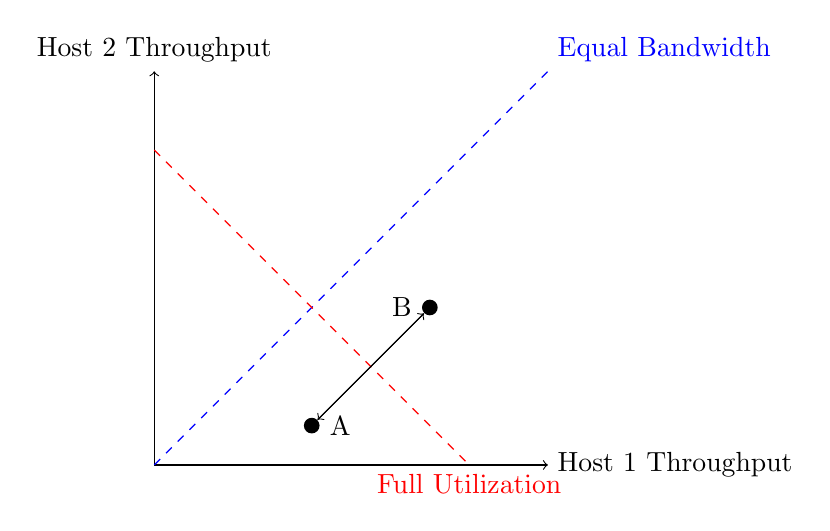
\begin{tikzpicture}[scale=1.0]
        % Axis
        \draw[->] (0,0) -- (5,0) node[right] {Host 1 Throughput};
        \draw[->] (0,0) -- (0,5) node[above] {Host 2 Throughput};
        % Equal Bandwidth Line
        \draw[dashed, blue] (0,0) -- (5,5) node[above right] {Equal Bandwidth};
        % Full Utilization Line
        \draw[dashed, red] (0,4) -- (4,0) node[below] {Full Utilization};
        % Host 1
        \node[label={180:{B}}, circle, fill, inner sep=2pt] (B) at (3.5,2) {};
        % Host 2
        \node[label={0:{A}}, circle, fill, inner sep=2pt] (A) at (2,0.5) {};
        \draw[->] (A) -- (B);
        \draw[->] (B) -- (A);
\end{tikzpicture}


\subsubsection{In Section 3.5.4, we discussed the doubling of the timeout interval after a timeout event. This mechanism is a form of congestion control. Why does TCP need a window-based congestion-control mechanism (as studied in  Section 3.7) in addition to this doubling-timeout-interval mechanism? (P42)}

TCP's use of pipelining allows the sender to have multiple outstanding unacknowledged segments. While a stop-and-wait protocol could rely on doubling the timeout interval as a congestion control mechanism, TCP's pipelining means this approach wouldn't suffice. Even with a doubled timeout interval, TCP can still transmit a large number of packets into a congested network. Thus, a congestion-control mechanism is necessary to manage the flow of data from the application when signs of network congestion arise.



\subsubsection{Host A is sending an enormous file to Host B over a TCP connection. Over this connection there is never any packet loss and the timers never expire. Denote the transmission rate of the link connecting Host A to the Internet by $R$ bps. Suppose that the process in Host A is capable of sending data into its TCP socket at a rate $S$ bps, where $S = 10 \cdot R$. Further suppose that the TCP receive buffer is large enough to hold the entire file, and the send buffer can hold only one percent of the file. What would prevent the process in Host A from continuously passing data to its TCP socket at rate S bps? TCP flow control? TCP congestion control? Or something else? Elaborate. (P43)}

It is not an issue that Host A can send data to its socket 10 times faster than it can transmit it from the socket to the network since the socket is large enough to hold the file. Since the socket of host B can only hold 1 percent of the file, then Host A is limited in its transmission from its socket by how fast host B can read data from its socket. This is controlled by defining the window size of host A tranmissions by TCP congestion control, however since this only limits the transmission from, and not to, host A's socket, there is nothing limiting host A from passing data to its socket at rate $S$.



\subsubsection{Consider sending a large file from a host to another over a TCP connection that has no loss. (P44)}

\textbf{a. Suppose TCP uses AIMD for its congestion control without slow start. Assuming \texttt{cwnd} increases by 1 MSS every time a batch of ACKs is received and assuming approximately constant round-trip times, how long does it take for \texttt{cwnd} increase from 6 MSS to 12 MSS (assuming no loss events)?} \\
No slow start means that \texttt{cwnd} increases by 1 MSS for every RTT. So it will take 6 RTTs for it to increase from 6 MSS to 12 MSS. \\
\\
\textbf{b. What is the average throughput (in terms of MSS and RTT) for this connection up through time = 6 RTT?}
Up to time 6 RTT we have that $1 + 2 + 3 + 4 + 5 + 6 = 21$ MSS have been received. Therefore the throughput up to time 6 RTT is $21/6 = 3.5$ MSS/RTT.



\subsubsection{Consider Figure 3.54. Suppose that at $t_3$, the sending rate at which congestion loss next occurs drops to $0.75 \cdot W_{\max}$ (unbeknownst to the TCP senders, of course). Show the evolution of both TCP Reno and TCP CUBIC for two more rounds each (Hint: note that the times at which TCP Reno and TCP CUBIC react to congestion loss may not be the same anymore). (P45)}

We have that $W_{\max}$ is the congestion window size at which loss last occurred. TCP Reno sets $\texttt{ssthresh} = W_{\max}/2$, sets $\texttt{cwnd} = \texttt{ssthresh} + 3$ MSS (we assume congestion loss is detected by tripple ACK as in figure 3.54) and after quick recovery starts the congestion avoidance phase. Therefore at $t_3 + RTT$ TCP Reno will have set $\texttt{cwnd} = W_{\max}/2 + 3$ and at $t_3 + 2 RTT$ it sets $\texttt{cwnd} = W_{\max}/2 + 4$. \\
\\
TCP Cubic will half the sending rate so that $\texttt{cwnd} =  W_{\max}/2$. TCP Cubic expects loss at time $K$ where $\texttt{cwnd} = 0.75 W_{\max}$ and will set $\texttt{cwnd}_t$ to a cube function of the distance between $t$ and $K$.



\subsubsection{Consider Figure 3.54 again. Suppose that at $t_3$, the sending rate at which congestion loss next occurs increases to $1.5 \cdot Wmax$. Show the evolution of both TCP Reno and TCP CUBIC for at two more rounds each (Hint: see the hint in P45). (P46)}

TCP Reno keep sending in the congestion avoidance phase such that at time $t_3 + RTT$ we have $\texttt{cwnd} = W_{\max}/2 + 1$ and at $t_3 + 2 RTT$ we have $\texttt{cwnd} = W_{\max}/2 + 2$. \\
\\
TCP Cubic expects loss at time $K$ where $\texttt{cwnd} = 1.5 W_{\max}$ and will set $\texttt{cwnd}_t$ to a cube function of the distance between $t$ and $K$.


\subsubsection{Recall the macroscopic description of TCP throughput. In the period of time from when the connection's rate varies from $W/(2 \cdot RTT)$ to $W/RTT$, only one packet is lost (at the very end of the period). (P47)}

\textbf{a. Show that the loss rate (fraction of packets lost) is equal to}
\begin{equation*}
    L = \text{loss rate} = \frac{1}{\frac{3}{8} W^2 + \frac{3}{4}W}
\end{equation*}
\\
The number of packets sent before packet loss, i.e. before $W/(2 \cdot RTT)$ increases to $W/RTT$ can, because of the linear increase in congestion avoidance, be expressed by 
\begin{equation*}
\begin{split}
    \frac{W}{2}+\left(\frac{W}{2}+1\right)+\cdots+W & =\sum_{n=0}^{W / 2}\left(\frac{W}{2}+n\right) \\
    & =\left(\frac{W}{2}+1\right) \frac{W}{2}+\sum_{n=0}^{W / 2} n \\
    & =\left(\frac{W}{2}+1\right) \frac{W}{2}+\frac{W / 2(W / 2+1)}{2} \\
    & =\frac{W^2}{4}+\frac{W}{2}+\frac{W^2}{8}+\frac{W}{4} \\
    & =\frac{3}{8} W^2+\frac{3}{4} W
\end{split}
\end{equation*} 
Since 1 packet is lost every time this amount of packets has been sent we have that the loss rate is
\begin{equation*}
    \frac{1}{\frac{3}{8} W^2+\frac{3}{4} W}
\end{equation*}
\\
\textbf{b. Use the result above to show that if a connection has loss rate $L$, then its average rate is approximately given by}
\begin{equation*}
    \approx \frac{1.22 \cdot MSS}{RTT \sqrt{L}}
\end{equation*}
\\
For large $W$ we have that the quadratic term dominates such that we can approximate the loss rate by 
\begin{equation*}
    L \approx \frac{1}{\frac{3}{8}W^2} = \frac{8}{3W^2}  
\end{equation*}
and express $W$ by 
\begin{equation*}
\begin{split}
    \frac{3L}{8} &\approx \frac{1}{W^2} \\
    W^2 &\approx \frac{8}{3L} \\
    W &\approx \sqrt{\frac{8}{3L}}
\end{split}
\end{equation*}
We have that \cite{kr} states that in exactly these settings we have that the average throughput is $\frac{3}{4}W/RTT$, inserting our value for $W$ (which is in the units of MSS) we get
\begin{equation*}
    \frac{\frac{3}{4} \sqrt{\frac{8}{3L}} MSS}{RTT} = \frac{\frac{3}{4} \sqrt{\frac{8}{3}} \frac{1}{\sqrt{L}} MSS}{RTT} = \frac{1.22 MSS}{RTT \sqrt{L}}
\end{equation*}



\subsubsection{Consider that only a single TCP (Reno) connection uses one 54 Mbps wireless link which does not buffer any data. Suppose that this link is the only congested link between the sending and receiving hosts. Assume that the TCP sender has a huge file to send to the receiver and the receiver's receive buffer is much larger than the congestion window. We also make the following assumptions: each TCP segment size is 536 bytes; the two-way propagation delay of this connection is 6 msec; and this TCP connection is always in congestion avoidance phase, that is, ignore slow start. (P48)}

\textbf{a. What is the maximum window size (in segments) that this TCP connection can achieve?} \\
Since the receiver buffer is larger than the congestion window then packet loss can only occur in the link, which happens as soon as queuing occurs since it does not buffer. Therefore the maximum window size must be set so the hosts do not send faster than the link's capacity. \\
\\
Sending at link capacity will mean that 
\begin{equation*}
\begin{split}
    \frac{W \cdot MSS}{RTT} &= 54 \, \text{Mbps} \\
    W &= \frac{RTT}{MSS} 54 \, \text{Mbps}
\end{split}
\end{equation*}
We have that $MSS = 536 \cdot 8$ bits and that $RTT = 2 \cdot 6 \cdot 10^{-3}$ seconds. Inserting these values we can determine $W$ by
\begin{equation*}
\begin{split}
    W &= \frac{12 \cdot 10^{-3} \, \text{s}}{536 \cdot 8 \, \text{bits}} 54 \cdot 10^6 \, \text{bits/s} \\
    &= 151.12
\end{split}
\end{equation*}
Flooring this value to make in an integer that does not go over the link capacity results in a maximum window size of $W = 151$ MSS. \\
\\
\textbf{b. What is the average window size (in segments) and average throughput (in bps) of this TCP connection?} \\
We have that the window will vary from $W/2$ (which is set on loss and increase linearly) to $W$. The average window size is therefore 
\begin{equation*}
    \overline{W} = \frac{W/2 + W}{2} = \frac{W}{4} + \frac{W}{2} = \frac{3}{4} W = \frac{3}{4} 151 = 113.25
\end{equation*}
\\
The average throughput $\overline{T}$ will can be expressed by
\begin{equation*}
    \overline{T} = \frac{\overline{W} \cdot MSS}{RTT} = \frac{113.25 \cdot 536 \cdot 8 \, \text{bits}}{12 \cdot 10^{-3} \, \text{s}} = 40.468 \cdot 10^6 \, \text{bits/s}
\end{equation*}
\\
\textbf{c. How long would it take for this TCP connection to reach its maximum window again after recovering from a packet loss?} \\
This is equivalent to the time it takes to increase the window size from $W/2$ to $W$ which can be expressed as
\begin{equation*}
    \lr{W - W/2} RTT = W/2 \cdot RTT  = \frac{151}{2} \cdot 12 \cdot 10^{-3} \, \text{s} = 0.906 \, \text{s}
\end{equation*}
since the window size increases by 1 MSS every RTT.

\subsubsection{Consider the scenario described in the previous problem. Suppose that the 10 Mbps link can buffer a finite number of segments. Argue that in order for the link to always be busy sending data, we would like to choose a buffer size that is at least the product of the link speed C and the two-way propagation delay between the sender and the receiver. (P49)}


\subsubsection{Repeat Problem 48, but replacing the 54 Mbps link with a 100 Gbps link and an RTT of 60 ms. Note that in your answer to part c, you will realize that it takes a very long time for the congestion window size to reach its maximum window size after recovering from a packet loss. Can you consider solutions for this? (P50)}


\subsubsection{Let $T$ (measured by RTT) denote the time interval that a TCP connection takes to increase its congestion window size from $W/2$ to $W$, where $W$ is the maximum congestion window size. Argue that $T$ is a function of TCP's  average throughput. (P51)}


\subsubsection{Consider a simplified TCP's AIMD algorithm where the congestion window size is measured in number of segments, not in bytes. In additive increase, the congestion window size increases by one segment in each RTT. In multiplicative decrease, the congestion window size decreases by half (if the result is not an integer, round down to the nearest integer). Suppose that two TCP connections, C1 and C2, share a single congested link of speed 30 segments per second. Assume that both C1 and C2 are in the congestion avoidance phase. Connection C1's RTT is 50 msec and connection C2's RTT is 100 msec. Assume that when the data rate in the link exceeds the link's speed, all  TCP connections experience data segment loss. (P52)}

\textbf{a. If both $C_1$ and $C_2$ at time $t_0$ have a congestion window of 10 segments, what are their congestion window sizes after 1000 msec?} \\
\\
\textbf{b. In the long run, will these two connections get the same share of the band-width of the congested link? Explain.}


\subsubsection{Consider the network described in the previous problem. Now suppose that the two TCP connections, C1 and C2, have the same RTT of 100 msec.  Suppose that at time $t_0$, C1's congestion window size is 15 segments but C2's congestion window size is 10 segments. (P53)}

\textbf{a. What are their congestion window sizes after 2200 msec?} \\
\\
\textbf{b. In the long run, will these two connections get about the same share of the bandwidth of the congested link?} \\
\\
\textbf{c. We say that two connections are synchronized, if both connections reach their maximum window sizes at the same time and reach their minimum window sizes at the same time. In the long run, will these two connections get synchronized eventually? If so, what are their maximum window sizes?} \\
\\
\textbf{d. Will this synchronization help to improve the utilization of the shared link? Why? Sketch some idea to break this synchronization.} \\


\subsubsection{Consider a modification to TCP's congestion control algorithm. Instead of additive increase, we can use multiplicative increase. A TCP sender increases its window size by a small positive constant a (0 < a < 1) whenever it receives a valid ACK. Find the functional relationship between loss rate L and maximum congestion window $W$. Argue that for this modified TCP, regardless of TCP's average throughput, a TCP connection always spends the same amount of time to increase its congestion window size from $W/2$ to $W$. (P54)}


\subsubsection{In our discussion of TCP futures in Section 3.7, we noted that to achieve a throughput of 10 Gbps, TCP could only tolerate a segment loss probability of $2 \cdot 10^{-10}$ (or equivalently, one loss event for every 5,000,000,000 segments). Show the derivation for the values of $2 \cdot 10^{-10}$ (1 out of 5,000,000) for the RTT and MSS values given in Section 3.7. If TCP needed to support a  100 Gbps connection, what would the tolerable loss be? (P55)}


\subsubsection{In our discussion of TCP congestion control in Section 3.7, we implicitly assumed that the TCP sender always had data to send. Consider now the case that the TCP sender sends a large amount of data and then goes idle (since it has no more data to send) at $t_1$. TCP remains idle for a relatively long period of time and then wants to send more data at $t_2$. What are the advantages and disadvantages of having TCP use the cwnd and ssthresh values from t1when starting to send data at $t_2$? What alternative would you recommend? Why? (P56)}


\subsubsection{In this problem, we investigate whether either UDP or TCP provides a degree of end-point authentication. (P57)}

\textbf{a. Consider a server that receives a request within a UDP packet and responds to that request within a UDP packet (for example, as done by a DNS server). If a client with IP address X spoofs its address with address Y, where will the server send its response?} \\
The server uses the source IP address in the received UDP packet to determine where to send the response. Since the packet appears to come from address Y, the server will send its response to the spoofed address Y. \\
\\
\textbf{b. Suppose a server receives a SYN with IP source address Y, and after responding with a SYNACK, receives an ACK with IP source address Y with the correct acknowledgment number. Assuming the server chooses a random initial sequence number and there is no ''man-in-the-middle,'' can the server be certain that the client is indeed at Y (and not at some other address X that is spoofing Y)?} \\
If someone was spoofind the Y address then they would not receive the SYNACK, which was sent to address Y along with the random sequence number. This means that the host at address Y would not send back an ACK since this host has not initialzed a three-way-handshake with SYN. If the spoofer were able to appropriately time an ACK to the server then they would still not be able to know the random sequence number (since we assume no man-in-the-middle to intecept this number). Therefore receiving an ACK with the correct sequence number ensures that the server can be certain that the client is indeed Y, so the answer is yes.

\subsubsection{In this problem, we consider the delay introduced by the TCP slow-start phase. Consider a client and a Web server directly connected by one link of rate $R$. Suppose the client wants to retrieve an object whose size is exactly equal to 15 $S$, where $S$ is the maximum segment size (MSS). Denote the round-trip time between client and server as RTT (assumed to be constant). Ignoring protocol headers, determine the time to retrieve the object (including TCP connection establishment) when: (P58)}

\textbf{a. $4 S/R > S/R + RTT > 2 S/R$} \\
\\
\textbf{b. $S/R + RTT > 4 S/R$} \\
\\
\textbf{c. $S/R > RTT$} \\
